\documentclass[10pt]{article}
\usepackage{tocloft}
\usepackage[utf8]{inputenc}
% \usepackage{hyperref}
\usepackage{geometry}

% Page Dimensions
\geometry{
  a4paper,
  total={170mm,257mm},
  left=10mm,
  top=15mm,
  right=10mm,
  bottom=13mm
}

\usepackage{graphicx}
\usepackage{titling}
\usepackage{fancyhdr}
\usepackage{titlesec}
\usepackage{wrapfig}
\usepackage{graphicx}
\usepackage{comment}
\usepackage[title,toc,titletoc,page]{appendix}
\usepackage{bold-extra}
\usepackage[scaled=0.85]{beramono}
\usepackage{enumitem}
\usepackage{multicol}
\usepackage{array}
\usepackage{mathtools,amssymb}
\usepackage[hidelinks]{hyperref}
%  Header for maths
\usepackage{amsmath}
\usepackage{amsfonts}
\usepackage{amssymb}
\usepackage{float}
\usepackage{fancyhdr}
\usepackage{lastpage}
\usepackage{pgfplots}
% \pgfplotsset{compat=1.18}
\usepackage{pgfplotstable}


% Section formatting
\titleformat{\section}
  {\normalfont\large\bfseries}
  {\thesection}
  {.5em}
  {}

% Subsection formatting
\titleformat{\subsection}
  {\normalfont\large\bfseries}
  {\thesubsection}
  {1em}
  {}

% Subsubsection formatting
\titleformat{\subsubsection}
  {\normalfont\normalsize\bfseries}
  {\thesubsubsection}
  {1em}
  {}

% Section spacing
\titlespacing*{\section}
  {0pt} % Left margin
  {1ex plus .1ex minus .1ex} % Space before section
  {0.5ex plus .1ex minus .1ex} % Space after section

% Subsection spacing
\titlespacing*{\subsection}
  {0pt} % Left margin
  {0.5ex plus .1ex minus .1ex} % Space before subsection
  {0.25ex plus .1ex minus .1ex} % Space after subsection

% Subsubsection spacing
\titlespacing*{\subsubsection}
  {0pt} % Left margin
  {0.5ex plus .1ex minus .1ex} % Space before subsubsection
  {0.25ex plus .1ex minus .1ex} % Space after subsubsection

\title{Analysis of Garbage Collection in Lua}
\author{Bratin Mondal}

\fancypagestyle{plain}{
    \fancyhf{}
    \fancyhead[L]{Analysis of Garbage Collection in Lua}
    \fancyhead[R]{Bratin Mondal}
}

\makeatletter
\def\@maketitle{%
  \newpage
  \null
  \begin{center}%
    {\LARGE \@title \par}%
  \end{center}%
  \par
  }
\makeatother

\usepackage{lipsum}  % Remove or replace with actual content
\usepackage{cmbright}

% No spacing between items in itemize
\usepackage{enumitem}
\setlist{nosep} % Removes extra space in lists

%  Reduce the font size of the document
\renewcommand{\normalsize}{\small}
\setlist[enumerate,1]{itemsep=0pt, parsep=0pt, topsep=0pt, partopsep=0pt}

\begin{document}

\maketitle

\noindent

\begin{flushleft}
    \textbf{Name:} Bratin Mondal \hfill \textbf{Course Code:} CS60203 \\
    \textbf{Roll Number:} 21CS10016 \hfill \textbf{Course Name:} Design Optimization of Computing Systems
\end{flushleft}

\section{Introduction}
This report discusses the variations of garbage collection algorithms used in Lua, analyzed after running them on different test benches.

\section{Percentage of Instructions Consumed by Garbage Collection}
\begin{table}[h]
    \centering
    \begin{tabular}{|c|c|}
        \hline
        \textbf{Garbage Collection Algorithm} & \textbf{Percentage of Instructions Consumed by Garbage Collection} \\
        \hline
        \texttt{full gc} & 21.89\% \\
        \texttt{incremental gc} & 19.87\% \\
        \texttt{generational gc} & 17.08\% \\
        \hline
    \end{tabular}
    \caption{Percentage of Instructions Consumed by Different Garbage Collection Algorithms}
    \label{tab:percentage_instructions_gc}
\end{table}

\subsection{Analysis}
The analysis of the results shows that the \texttt{full gc} algorithm consumes the highest percentage of instructions, followed by \texttt{incremental gc}, and finally \texttt{generational gc}.

\subsubsection{Full GC}
The \texttt{full gc} algorithm has the highest instruction consumption:
\begin{enumerate}
    \item The full garbage collection was executed at the end when all memory allocations had been completed, meaning the collector had to traverse a large set of objects to determine which were garbage.
    \item The \texttt{sweeplist} function, responsible for traversing and freeing garbage objects, consumed \textbf{21.50\%} of the total instructions used by the garbage collector. Out of this, \textbf{18.99\%} was consumed by the \texttt{freeobj} function, indicating that the collector spent most of its time freeing a large number of objects.
\end{enumerate}

\subsubsection{Incremental GC}
The \texttt{incremental gc} algorithm consumes the second-highest percentage of instructions:
\begin{enumerate}
    \item The incremental garbage collector operated in multiple cycles, reducing the number of objects to be traversed in each cycle.
    \item The \texttt{atomic} function was executed \textbf{20} times, completing \textbf{20} full cycles of garbage collection. 
    \item The \texttt{singlestep} function was called \textbf{80} times, resulting in 80 pauses during execution, each completing a different step of the garbage collection process.
    \item During these pauses, the \texttt{atomic} function consumed only \textbf{0.03\%} of the total instructions, as the testbench had no weak tables or finalizers, which are typically handled by the \texttt{atomic} function.
    \item The \texttt{propagatemark} function consumed \textbf{8.80\%} of the total instructions and was called \textbf{867,609} times, with only \textbf{2,331} calls originating from the \texttt{atomic} function. This indicates that the marking task was well-distributed across cycles.
    \item The \texttt{sweepstep} function consumed \textbf{8.78\%} of the total instructions, with \textbf{8.76\%} used by the \texttt{sweeplist} function. This is lower than the \texttt{full gc} algorithm's consumption, as the incremental collector traversed a smaller set of objects in each cycle.
\end{enumerate}

\subsubsection{Generational GC}
The \texttt{generational gc} algorithm is the most efficient in terms of instruction consumption:
\begin{enumerate}
    \item The generational garbage collector, similar to the incremental one, operated in multiple cycles, further reducing the objects traversed per cycle.
    \item The \texttt{luaC\_step} function was called \textbf{22} times, indicating \textbf{22} pauses for garbage collection.
    \item The \texttt{sweepgen} function was called \textbf{30} times, completing \textbf{6} young generational collections (5 calls are made for each young generational collection) only traversing the young generation objects. This optimized approach reduced the instruction consumption compared to the incremental garbage collector.
    \item The \texttt{atomic} function was called \textbf{21} times, consuming \textbf{8.30\%} of the total instructions, higher than the incremental garbage collector. This difference arises because the generational collector checks the whole object set during major collections, while the incremental collector only traverses the gray objects.
    \item The \texttt{propagatemark} function consumed \textbf{7.97\%} of the total instructions and was called \textbf{788,835} times, with \textbf{788,786} calls from the \texttt{atomic} function, indicating a significant amount of marking done during each pause.
    \item The \texttt{sweepstep} function consumed \textbf{8.75\%} of the total instructions, with \textbf{8.73\%} used by the \texttt{sweeplist} function. This is much lower than the \texttt{full gc} and slightly lower than the \texttt{incremental gc}, as the generational collector also traversed fewer objects per cycle.
\end{enumerate}

\subsection{Conclusion}
The analysis reveals that the generational and incremental garbage collectors are more efficient than the full garbage collector. The generational collector has a slight edge due to its separation of objects into young and old generations, allowing for frequent minor collections and reducing instruction consumption. The incremental garbage collector, while also efficient, consumes slightly more instructions due to its multi-cycle approach. The full garbage collector is the least efficient, as it must traverse the entire object set in a single cycle, leading to higher instruction consumption.


\section{TestBench with Different Parameters}
\begin{table}[H]
  \centering
  \begin{tabular}{|c|c|c|c|}
      \hline
      \textbf{m,n} & \textbf{Full GC} & \textbf{Incremental GC} & \textbf{Generational GC} \\
      \hline
      \texttt{100,100} & 21.76\% & 16.64\% & 15.07\% \\
      \texttt{500,100} & 21.87\% & 18.48\% & 15.48\% \\
      \texttt{1000,100} & 21.89\% & 19.87\% & 17.08\% \\
      \texttt{5000,100} & 27.81\% & 15.03\% & 18.43\% \\
      \hline
  \end{tabular}
  \caption{Percentage of Instructions Consumed by Garbage Collection in Different TestBenches}
  \label{tab:percentage_instructions_gc_testbenches}
\end{table}

\begin{figure}[H]
  \centering
  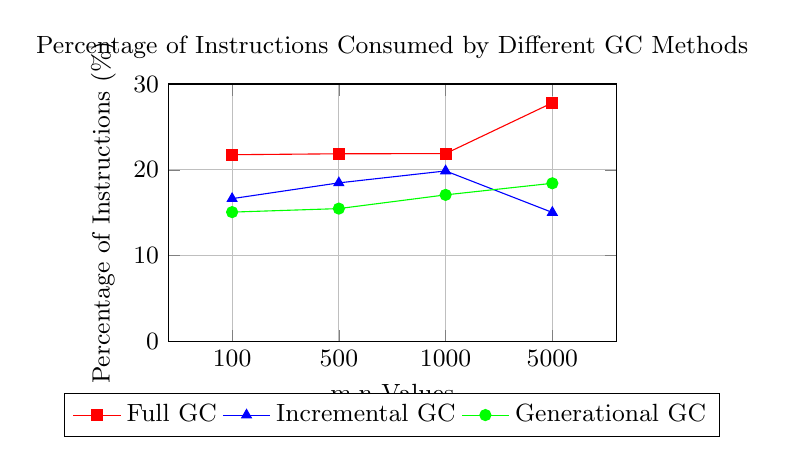
\begin{tikzpicture}
      \begin{axis}[
          width=0.6\textwidth, % Reduce width
          height=0.4\textwidth, % Reduce height
          enlarge x limits=0.2,
          legend style={at={(0.5,-0.2)}, anchor=north, legend columns=-1}, % Adjust legend position
          symbolic x coords={100,500,1000,5000},
          xtick=data,
          ymin=0, ymax=30,
          ylabel={Percentage of Instructions (\%)},
          xlabel={m,n Values},
          grid=major,
          ymajorgrids=true,
          tick label style={font=\small},
          mark options={solid},
          title={Percentage of Instructions Consumed by Different GC Methods}
      ]
      \addplot[color=red, mark=square*] coordinates {(100,21.76) (500,21.87) (1000,21.89) (5000,27.81)};
      \addplot[color=blue, mark=triangle*] coordinates {(100,16.64) (500,18.48) (1000,19.87) (5000,15.03)};
      \addplot[color=green, mark=*] coordinates {(100,15.07) (500,15.48) (1000,17.08) (5000,18.43)};
      \legend{Full GC, Incremental GC, Generational GC}
      \end{axis}
  \end{tikzpicture}
  \caption{Percentage of Instructions Consumed by Different Garbage Collection Methods in Various TestBenches.}
  \label{fig:percentage_instructions_gc_testbenches}
\end{figure}

We analyze the percentage of instructions consumed by garbage collection in different testbenches with varying \texttt{m,n} values for all three garbage collection algorithms.

\subsection{Analysis}
\subsubsection{Full GC}
\begin{itemize}
    \item Full GC consistently consumes the highest percentage of instructions compared to the other garbage collection methods.
    \item From testbench 1 to testbench 3, Full GC's instruction consumption increases slightly. This indicates that as the matrix size grows, Full GC starts to consume a slightly higher percentage of instructions. However, for lower values of \texttt{m,n}, the difference is negligible, suggesting stability over a smaller range of matrix sizes.
    \item In testbench 4, Full GC's instruction consumption increases significantly to \textbf{27.81\%} from \textbf{21.89\%} in testbench 3. This sharp increase highlights that the overhead for Full GC grows significantly with larger matrix sizes, likely due to the increased amount of memory and objects being managed.
\end{itemize}
In essence, Full GC is manageable for smaller to moderately sized datasets, but its cost escalates significantly with larger datasets. This is the main reason why Full GC is not suitable for real-time applications or large-scale systems.

\subsubsection{Incremental GC}
\begin{itemize}
    \item Incremental GC consumes a moderate percentage of instructions, performs second-best on testbenches 1 to 3 and best on testbench 4.
    \item In testbench 1, Incremental GC consumes \textbf{16.64\%} of instructions. There were \textbf{14} calls to the \texttt{luaC\_step} function and \textbf{14} calls to the \texttt{atomic} function. This indicates a total of \textbf{14} cycles of garbage collection. Although Incremental GC performed better than Full GC, the distribution of marking and sweeping tasks was not optimally managed across pauses.
    \item In testbench 2, Incremental GC consumes \textbf{18.48\%} of instructions. The increase in percentage is mainly due to managing a larger amount of memory and objects. The number of calls to \texttt{luaC\_step} increased significantly to \textbf{42}, while calls to the \texttt{atomic} function increased slightly to \textbf{18}. This suggests that marking and sweeping tasks were not perfectly distributed across pauses. Despite the higher instruction consumption compared to testbench 1, Incremental GC better managed the increased matrix size by distributing tasks across pauses.
    \item In testbench 3, Incremental GC consumes \textbf{19.87\%} of instructions. The number of calls to \texttt{luaC\_step} increased to \textbf{80}, and calls to the \texttt{atomic} function increased to \textbf{20}. While the percentage of instructions consumed rose slightly compared to testbench 2, the distribution of marking and sweeping tasks was improved.
    \item In testbench 4, Incremental GC consumes \textbf{15.03\%} of instructions. This is the lowest percentage of instructions consumed by Incremental GC across all testbenches, and it represents the best performance among all garbage collection algorithms for this testbench. The number of calls to \texttt{luaC\_step} increased to \textbf{276}, while calls to the \texttt{atomic} function increased only to \textbf{23}. This indicates that Incremental GC managed the increased workload more efficiently as the matrix size grew.
\end{itemize}
Incremental GC aims to interleave garbage collection steps with program execution using tri-color marking schemes and barriers. This approach updates the status of objects efficiently, reducing the time spent on marking by only traversing gray objects managed by barriers. For larger datasets, Incremental GC demonstrates improved performance compared to other garbage collection algorithms.

\subsubsection{Generational GC}
\begin{itemize}
  \item Generational GC performs best on testbenches 1 to 3, consuming the least percentage of instructions among all GC types, and second-best on testbench 4, where Incremental GC outperforms it slightly.
  
  \item The percentage of instructions consumed by Generational GC increases slightly from testbench 1 to testbench 2, rising from \textbf{15.07\%} to \textbf{15.48\%}. However, a more significant increase is observed from testbench 2 to testbench 3, where it jumps from \textbf{15.48\%} to \textbf{17.08\%}. This upward trend continues from testbench 3 to testbench 4, where the consumption rises from \textbf{17.08\%} to \textbf{18.43\%}. This pattern suggests that Generational GC is highly efficient for smaller matrices, but its efficiency diminishes as the matrix size grows due to the increased complexity in managing larger memory footprints.

  \item Although Generational GC is designed to optimize memory management by segregating objects into young and old generations, it struggles with larger matrices. As the number of objects in the old generation increases, the collector needs to perform more extensive and frequent collections, which involve traversing a large number of objects. This comprehensive traversal becomes more costly, leading to a noticeable decline in performance on testbench 4 compared to the incremental garbage collector.

  \item Larger matrices increase the memory footprint, leading to more frequent and intensive GC activity. As the workload grows, managing the old generation becomes more demanding, resulting in higher instruction consumption and reduced GC efficiency.
\end{itemize}
Generational GC is efficient for smaller datasets but struggles with larger matrices due to the increased complexity of managing larger memory footprints. The generational approach is designed to optimize memory management by segregating objects into young and old generations, but it becomes less effective as the workload grows, leading to higher instruction consumption and reduced efficiency.

\subsection{Conclusion}
The analysis shows that Incremental GC is the most efficient for larger datasets, consuming the least instructions in testbench 4. Generational GC performs well with smaller datasets but becomes less efficient as matrix size increases, leading to higher instruction consumption. Full GC is the least efficient, with significant instruction costs for larger datasets. Incremental GC's interleaved approach and tri-color marking schemes make it better suited for managing larger workloads compared to other GC algorithms. While Generational GC excels with smaller datasets, its efficiency declines with growing workloads.


\section{Analysis with Perf}
% Table 
The performance analysis of garbage collection algorithms using the \texttt{perf} tool is shown in Table below. The readings are average of 100 runs.

\begin{table}[H]
  \centering
  \begin{tabular}{|c|c|c|c|c|}
      \hline
      \textbf{Garbage Collection Algorithm} & \textbf{Branch Misses} & \textbf{Page Faults} & \textbf{Cache Misses} & \textbf{Instructions per Cycle} \\
      \hline
      \texttt{no gc} & 421,607 & 16,258 & 1,581,617 & 3.08 \\
      \texttt{full gc} & 413,775 & 16,258 & 1,582,313 & 3.04 \\
      \texttt{incremental gc} & 503,439 & 11,131 & 6,413,636 & 2.04 \\
      \texttt{generational gc} & 486,692 & 10,088 & 7,671,638 & 1.89 \\
      \hline
  \end{tabular}
  \caption{Performance Analysis of Garbage Collection Algorithms}
  \label{tab:performance_analysis_gc}
\end{table}


\subsection{Branch Misses}
\subsubsection{Importance}
\begin{enumerate}
  \item \textbf{Impact on Execution Flow:} GC algorithms often involve complex memory operations that can lead to unpredictable execution paths, challenging the branch predictor and potentially degrading performance.
  \item \textbf{Effect on Control Flow Predictability:} Frequent changes in the approach of the garbage collector during GC operations can reduce the accuracy of the branch predictor, increasing branch miss rates and leading to inefficiencies in CPU execution.
  \item \textbf{Correlation with Algorithm Complexity:} More complex GC algorithms with intricate memory management and object traversal logic tend to disrupt the branch predictor more frequently, resulting in higher branch miss rates and reduced performance.
\end{enumerate}

\subsubsection{Analysis}
\begin{enumerate}
  \item \textbf{No GC:} 
  \begin{itemize}
    \item \textbf{Branch Misses:} 421,607
    \item \textbf{Explanation:} The baseline measurement for branch misses shows minimal branch mispredictions due to stable execution paths. However, the branch miss rate is higher than in the Full GC scenario, possibly due to the \texttt{lua\_close} function's approach to freeing resources, which may introduce some unpredictability in the control flow.
  \end{itemize}

  \item \textbf{Full GC:} 
  \begin{itemize}
    \item \textbf{Branch Misses:} 413,775
    \item \textbf{Explanation:} Full GC shows a slight reduction compared to No GC. This is due to Full GC pausing the entire program for garbage collection only at the end. The collector's execution pattern during this pause is relatively stable and predictable, leading to fewer branch mispredictions, even lower than the baseline.
  \end{itemize}

  \item \textbf{Incremental GC:} 
  \begin{itemize}
    \item \textbf{Branch Misses:} 503,439
    \item \textbf{Explanation:} Incremental GC experiences the highest branch miss rate. This algorithm performs garbage collection in small, interleaved steps, leading to frequent switching between program execution and GC operations. This results in high unpredictability and more frequent branch mispredictions.
  \end{itemize}

  \item \textbf{Generational GC:} 
  \begin{itemize}
    \item \textbf{Branch Misses:} 486,692
    \item \textbf{Explanation:} Generational GC shows fewer branch misses than Incremental GC but more than Full GC. The complexity of managing object generations and making decisions about which objects to collect or promote adds some unpredictability to execution paths.
  \end{itemize}
\end{enumerate}

\subsection{Page Faults}
\subsubsection{Importance}
\begin{enumerate}
  \item \textbf{Memory Management:} Efficient garbage collection that reuses memory can reduce page faults and improve performance.
  \item \textbf{GC Impact on Memory:} Frequent memory access during GC operations can lead to increased page faults, especially if the GC algorithm does not consider memory locality.
  \item \textbf{Performance Implications:} Excessive page faults can degrade performance significantly due to slower disk I/O operations. Optimizing GC to minimize page faults is crucial for maintaining performance.
\end{enumerate}

\subsubsection{Analysis}
\begin{enumerate}
  \item \textbf{No GC:} 
  \begin{itemize}
    \item \textbf{Page Faults:} 16,258
    \item \textbf{Explanation:} The baseline scenario with no garbage collection shows a moderate level of page faults due to the application's own memory demands and system paging behavior.
  \end{itemize}

  \item \textbf{Full GC:} 
  \begin{itemize}
    \item \textbf{Page Faults:} 16,258
    \item \textbf{Explanation:} Full GC maintains the same page fault rate as No GC, as it involves stopping the entire application only at the end of the process, without significantly altering memory access patterns.
  \end{itemize}

  \item \textbf{Incremental GC:} 
  \begin{itemize}
    \item \textbf{Page Faults:} 11,131
    \item \textbf{Explanation:} Incremental GC results in fewer page faults compared to No GC and Full GC, indicating effective memory management by performing garbage collection in small steps that maintain memory locality.
  \end{itemize}

  \item \textbf{Generational GC:} 
  \begin{itemize}
    \item \textbf{Page Faults:} 10,088
    \item \textbf{Explanation:} Generational GC has the lowest page fault rate, showing effective memory management by segregating objects into generations and frequently collecting young objects to minimize paging.
  \end{itemize}
\end{enumerate}

\subsection{Cache Misses}
\subsubsection{Importance}
\begin{enumerate}
  \item \textbf{Memory Access Patterns:} GC algorithms that traverse large memory regions or have complex heuristics can lead to increased cache misses, unable to use the caching system effectively.
  \item \textbf{Performance Degradation:} Poor memory access patterns during GC can lead to increased cache misses, affecting overall performance.
\end{enumerate}

\subsubsection{Analysis}
\begin{enumerate}
  \item \textbf{No GC:} 
  \begin{itemize}
    \item \textbf{Cache Misses:} 1,581,617
    \item \textbf{Explanation:} The baseline performance with no garbage collection shows relatively low cache misses, indicating efficient memory access without GC overhead.
  \end{itemize}

  \item \textbf{Full GC:} 
  \begin{itemize}
    \item \textbf{Cache Misses:} 1,582,313
    \item \textbf{Explanation:} Full GC introduces a slight increase in cache misses compared to No GC. This increase is minimal, reflecting that the pause for GC may not significantly impact cache performance.
  \end{itemize}

  \item \textbf{Incremental GC:} 
  \begin{itemize}
    \item \textbf{Cache Misses:} 6,413,636
    \item \textbf{Explanation:} Incremental GC results in a significant increase in cache misses due to frequent switching between GC and program execution and accessing different memory regions during small GC steps which invalidates cache lines.
  \end{itemize}

  \item \textbf{Generational GC:} 
  \begin{itemize}
    \item \textbf{Cache Misses:} 7,671,638
    \item \textbf{Explanation:} Generational GC shows the highest number of cache misses due to frequent object promotion and the need to manage multiple generations, leading to extensive memory traffic outside the cache and incurs most cache misses.
  \end{itemize}
\end{enumerate}


\subsection{Instructions per Cycle (IPC)}
\subsubsection{Importance}
\begin{enumerate}
  \item \textbf{Impact of GC Overhead:} GC algorithms can introduce overhead that affects the CPU's ability to execute instructions efficiently avoiding stalls.
  \item \textbf{Performance Bottlenecks:} Lower IPC can signal performance bottlenecks caused by GC operations, such as increased branch mispredictions or cache misses.
\end{enumerate}

\subsubsection{Analysis}
\begin{enumerate}
  \item \textbf{No GC:} 
  \begin{itemize}
    \item \textbf{IPC:} 3.08
    \item \textbf{Explanation:} Without GC, the system achieves the highest IPC of 3.08, reflecting optimal CPU efficiency with no GC-induced overhead. The baseline performance is limited only by code execution and hardware capabilities.
  \end{itemize}

  \item \textbf{Full GC:} 
  \begin{itemize}
    \item \textbf{IPC:} 3.04
    \item \textbf{Explanation:} The IPC for Full GC is slightly lower than No GC, indicating a minor reduction in CPU efficiency due to the garbage collection overhead. The pause for Full GC at the end of the process introduces some overhead, leading to a small decrease in IPC compared to the baseline.
  \end{itemize}

  \item \textbf{Incremental GC:} 
  \begin{itemize}
    \item \textbf{IPC:} 2.04
    \item \textbf{Explanation:} Incremental GC significantly lowers IPC to 2.04 due to the overhead of managing garbage collection in small, incremental steps. This results in increased branch mispredictions and cache misses, reducing overall CPU efficiency.
  \end{itemize}

  \item \textbf{Generational GC:} 
  \begin{itemize}
    \item \textbf{IPC:} 1.89
    \item \textbf{Explanation:} Generational GC exhibits the lowest IPC of 1.89. The significant reduction in IPC is due to the high overhead associated with managing multiple generations of objects, leading to extensive memory traffic and inefficient CPU utilization.
  \end{itemize}
\end{enumerate}

\end{document}
